% ============================================================================================
% This is a LaTeX template used for the course
%
%  I M A G E   B A S E D   B I O M E T R I C S
%
% Faculty of Computer and Information Science
% University of Ljubljana
% Slovenia, EU
%
% You can use this template for whatever reason you like.
% If you have any questions feel free to contact
% ziga.emersic@fri.uni-lj.si
% ============================================================================================

\documentclass[9pt]{IEEEtran}

% basic
\usepackage[english]{babel}
\usepackage{graphicx,epstopdf,fancyhdr,amsmath,amsthm,amssymb,url,array,textcomp,svg,listings,hyperref,xcolor,colortbl,float,gensymb,longtable,supertabular,multicol,placeins}

 % `sumniki' in names
\usepackage[utf8x]{inputenc}

 % search and copy for `sumniki'
\usepackage[T1]{fontenc}
\usepackage{lmodern}
\input{glyphtounicode}
\pdfgentounicode=1

% tidy figures
\graphicspath{{./figures/}}
\DeclareGraphicsExtensions{.pdf,.png,.jpg,.eps}

% correct bad hyphenation here
\hyphenation{op-tical net-works semi-conduc-tor trig-gs}

% ============================================================================================

\title{\vspace{0ex} %
Ear Detector
\\ \large{Assignment \#2}\\ \normalsize{Image Based Biometrics 2020/21, Faculty of Computer and Information Science, University of Ljubljana}}
\author{ %
Jan~Joneš
\vspace{-4.0ex}
}

% ============================================================================================

\begin{document}

\maketitle

\begin{abstract}
In this report, I describe results of developing an ear detector.
First I describe detector architecture.
Then I present performance results.
\end{abstract}

\section{Introduction}
I developed a convolutional neural network (CNN) that can segment ears pixel-wise.
This network is intended for use in biometric pipeline.
The architecture has been developed from scratch based on my knowledge from deep learning course~\cite{npfl114}.
For training and evaluation, I have used AWE-W dataset~\cite{awe}.
Source code of both the model and this report can be found in GitHub repository~\cite{repo}.

\section{Methodology}
The chosen dataset is already split into training and testing subsets (750 and 250 images, respectively).
I have further subdivided the original training data into (actual) training and development subsets (500 and 250 images, respectively).
Both of these training subsets were used during development of the detector.
Testing data were used only during final evaluation.

All images are already resized to the same size ($480 \times 360$ pixels) in the dataset.
In order to use them easily in convolutional layers of the CNN, I have resized them to dimensions divisible by 32 ($480 \times 352$ pixels) during preprocessing.

The CNN uses pre-trained EfficientNet-B0 network~\cite{efficientNet} as encoder in U-Net-like architecture~\cite{unet} and custom decoder and segmentation head.
EfficientNet-B0 takes pixels as input and outputs them scaled down 32 times. The decoder uses transposed convolutions to scale these features back to the original resolution and employs skip layers to pass information from the corresponding layer of the encoder.

The encoder has its weights fixed to the pre-trained values. Only encoder's weights are trained. The CNN has 6.9 million trained parameters and 4.0 million fixed parameters.

\section{Results}
Nulla sodales, metus at faucibus iaculis, felis risus pulvinar erat, in pretium arcu ex sed elit. Cras ultrices felis in diam dictum interdum. Praesent in interdum dolor, ut varius massa. Integer non efficitur risus, nec dapibus dui. Nunc sollicitudin nibh in orci pretium, quis congue ligula faucibus. Vivamus fermentum leo ac euismod porta as shown in Figure~\ref{fig:plot1}.

\begin{figure}[h]
    \centering
    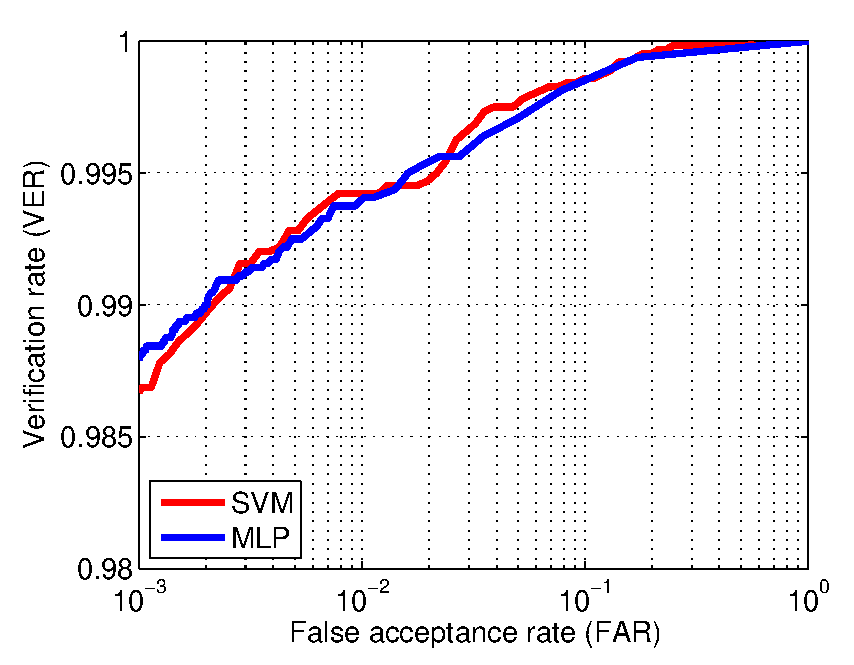
\includegraphics[width=1\columnwidth]{plot1}
    \caption{A nice plot showing something really cool and awesome.}
    \label{fig:plot1}
\end{figure}
 
Sed et enim non justo mattis finibus sed at felis. Phasellus vel nibh vehicula, consectetur lectus in, bibendum enim. Nam rutrum suscipit magna id maximus. Quisque posuere lorem vel ante viverra, ut euismod sapien pulvinar. Fusce vitae maximus nibh. Sed dignissim dignissim nunc eu finibus. In pulvinar purus nisl, et mattis magna pretium ac. Curabitur nec massa vel est eleifend cursus nec sed elit. Vestibulum at nibh felis. Sed porttitor ut turpis in tristique.

 \section{Conclusion}

Aenean tincidunt sodales ante et egestas. Nam consectetur nunc iaculis tincidunt egestas. Vivamus sagittis mi et vehicula facilisis. Phasellus semper volutpat gravida. Vestibulum vitae neque sed purus pharetra suscipit eget mollis dui. Morbi lobortis justo a lacus feugiat, et finibus eros tristique.

\bibliographystyle{IEEEtran}
\bibliography{bibliography}

\end{document}
